\documentclass[19pt,a4paper]{article}
\usepackage{xeCJK}
\usepackage{amsmath}
\setmainfont{STSong}
\usepackage{geometry}
\geometry{left=2.5cm,right=2.5cm,top=2.5cm,bottom=2.5cm}
\setlength{\parindent}{4em}
\usepackage{graphicx}
\title{算法作业4}
\author{孟妍廷2015202009}
\date{2017年10月15日}

\begin{document}
\maketitle

6.4-1\\
\indent 如图:
\begin{figure}[htbp]
 \centering
 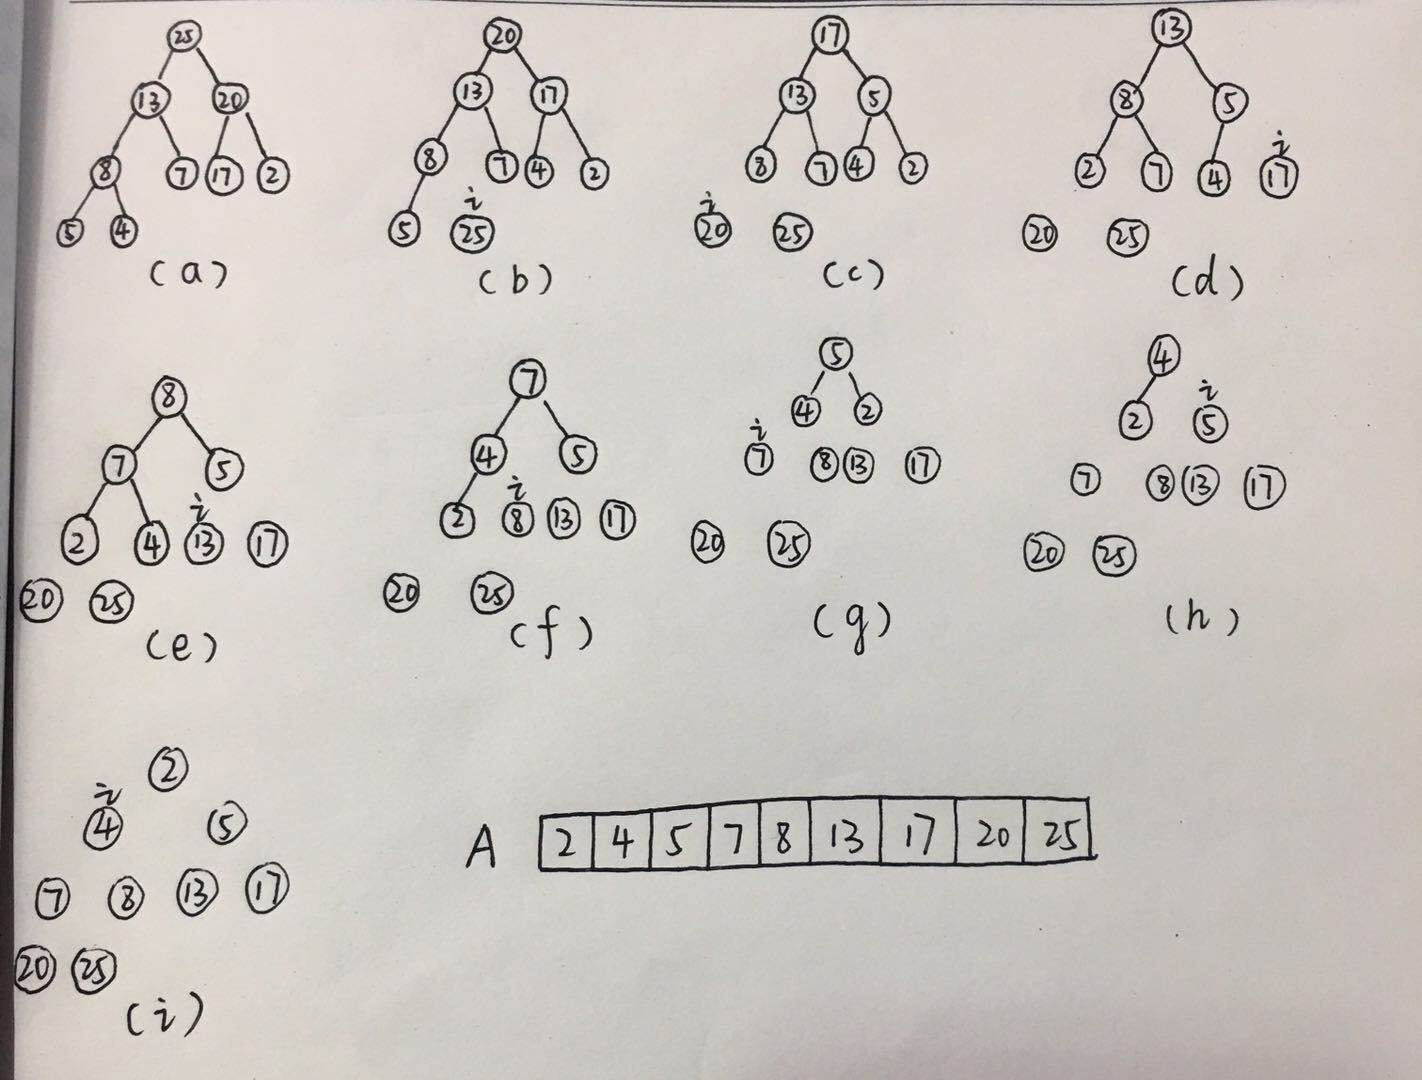
\includegraphics[scale=0.3]{1.jpeg}
\end{figure}\\
\\
\indent 7-5\\
\indent a.若中位数取到i,则等同于取两个数,一个小于i,一个大于i,表达式为:\\
$$p_i=\frac{(i-1)(n-i)}{c_n^3}$$
$$=\frac{6(i-1)(n-i)}{n(n-1)(n-2)}$$
\indent b.依题意可得:\\
$$p_{\frac{n+1}{2}}=P(x=A^\prime[\frac{n+1}{2}])$$
$$=\frac{6(\frac{n+1}{2}-1)(n-\frac{n+1}{2})}{n(n-1)(n-2)}$$
$$=\frac{3(n-1)}{2n(n-2)}$$
\indent 平凡实现的$p_{\frac{n+1}{2}}=\frac{1}{n}$,故增加了$\frac{n+1}{2n(n-2)}$\\
\indent 当$n\rightarrow\infty$时,\\
$$\lim_{n\to\infty}\frac{3(n-1)}{2n(n-2)}=0$$
\indent 因此几乎没有增加。\\
\indent c.依题意可得:\\
$$P=\int_{\frac{n}{3}}^{\frac{2n}{3}}  \frac{6(i-1)(n-i)}{n(n-1)(n-2)} di.$$
$$=\frac{6}{n(n-1)(n-2)}(\int_{\frac{n}{3}}^{\frac{2n}{3}}(n+1)idi-\int_{\frac{n}{3}}^{\frac{2n}{3}}ndi-\int_{\frac{n}{3}}^{\frac{2n}{3}}i^2di)$$
$$=\frac{13n^2-27n}{27(n-1)(n-2)}$$
\indent 与b同理,概率增加了$\frac{13n^2-27n}{27(n-1)(n-2)}-\frac{1}{n}$\\
\indent 进一步量化,当$n\rightarrow\infty$时,\\
$$\lim_{n\to\infty}\frac{13n^2-27n}{27(n-1)(n-2)}-\frac{1}{n}$$
$$=\lim_{n\to\infty}\frac{13n^2}{27(n-1)(n-2)}+0+0$$
$$\approx \frac{13}{27}$$
\indent d.证明:\\
\indent 最佳情况是每一次主元都取到了A[$\frac{n+1}{2}$]处(n为当前数组长度)\\
\indent 此时parttion()函数的代价是lgn,因此快排的代价是nlgn\\
\indent 故三数取中法的时间复杂度为$\Omega(nlgn)$,只影响了常数项\\


\end{document}